\begin{center}
 \begin{minipage}[b]{0.45\textwidth} 
\subsection*{General information}
Name: David Rasmussen \\
Address: Islands brygge 56b 1tv \\
Zip nr. 2300 Koebenhavn S \\
Phone number: 26325635 \\
E-mail: david2300@hotmail.com \\
Country: Danmark \\
Date of birth: 11/06/1995
\newline
 \end{minipage}
 \hfill
\begin{minipage}[b]{4.5cm}
 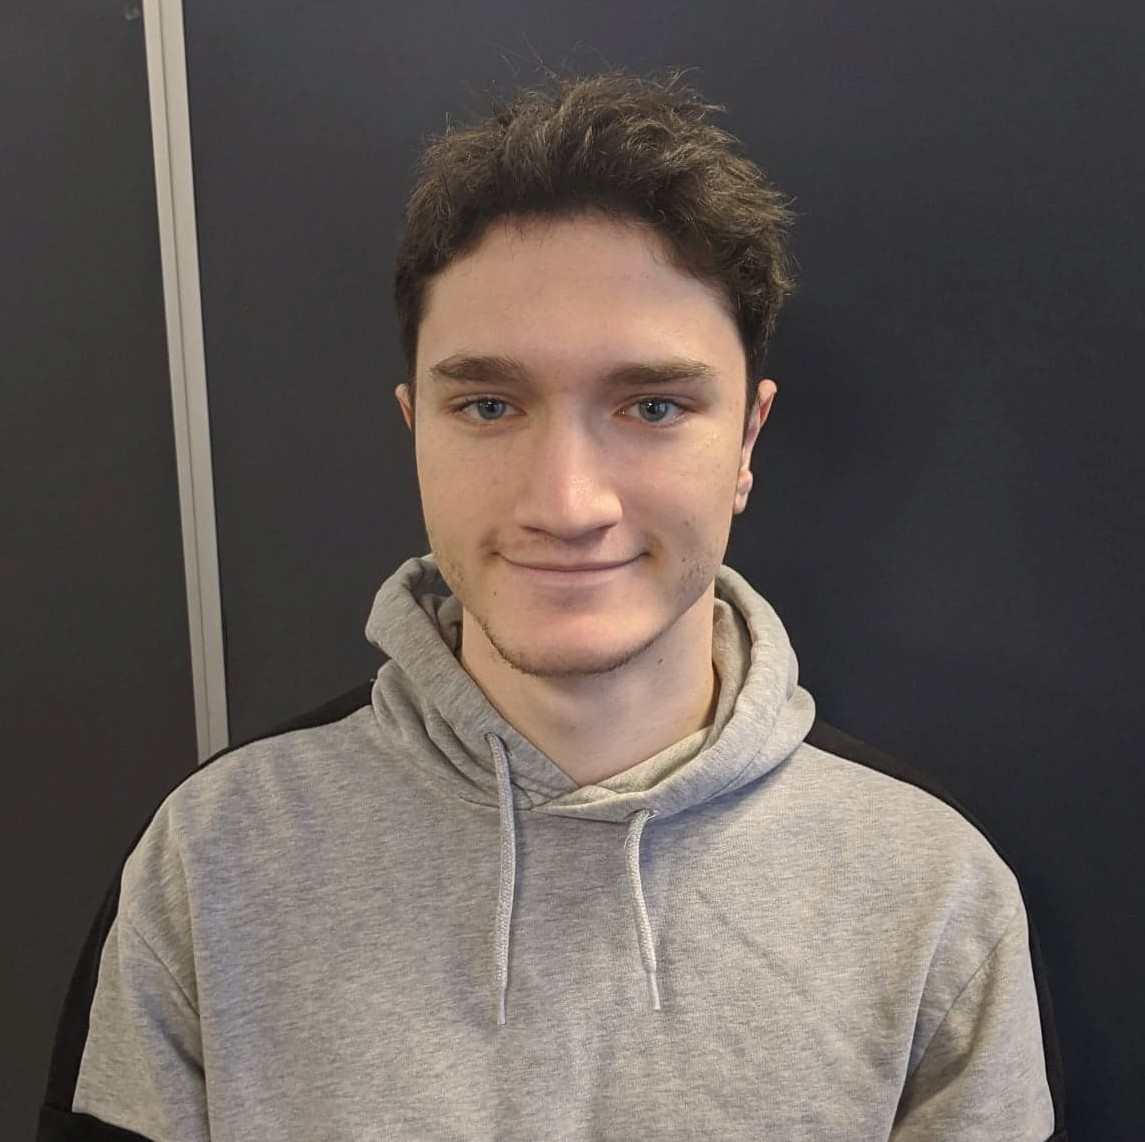
\includegraphics[height=4.25cm]{figures/Billede_af_David}
 \end{minipage}
 \end{center}

\section*{Work experience}
\begin{itemize}
\item 2010 - 2012 Netto - Sevice employee
\item 2012 - 2013 Bauhaus Valby - Salesman
\item 2013 - 2014 Q8 - Sales Assistant
\item 2016 - 2018 Elgiganten Glostrup - Cross operation 
\item 2018 - 2020 Concept - Client service 
\end{itemize}
\section*{Education}
\begin{itemize}
\item 2011 - 2014 HTX-Hilleroed, Biotech
\item 2015 - 2018 Aalborg university Bachelor of Software Engineering
\item 2018 - 2020 Aalborg university Master of Software Engineering
\end{itemize}

\section*{Background Information}
Took a highschool diploma in Biotechnology and chemistry: capable of doing PCR testing.\\Highschool exam project was using c sharp (unity) to make a game.\\Currently doing a bsc in engineering (software) at Aalborg university.\\University focuses on teamwork, so i have lots of experience with larger groups.\\Lots of skills in programming.\\Able to set up databases using SQL and net.\\Large interest in electronics. Done multiple projects.\\Capable of using machine learning using python. Also read a lot of statistics and probability theory to learn the theory behind it. Can use neural networks, to predict behavior.\\Proficient in C++.\\Mad my own website using HTML and CSS\\able to do mathamtical optimization using matlab.\\
